%Figure~\ref{figure:pipeline} depicts the summarized pipeline of the proposed method. This pipeline contains two main steps: first, the application of 1D-to-2D signal projections, where the 1D signal is transformed into a 2D image, and, then, the application of a \gls{CVC} algorithm to classify the quality of signal into reliable/not-reliable. The 1D-to-2D projection can be performed by using \gls{mtf}, \gls{rp}, or \gls{gaf} algorithms. 


%Moreover, the image aggregation of those three methods, \acrfull{PM}, was used in the scope of this work. It assigns the beforementioned projection methods images to each of the RGB channels. To the best of our knowledge, no previous work has considered a \gls{PM} yet.



%The signal projection approach can produce competitive results with state of art approaches, as using \acrshort{gaf} in combination with Vision Transformer \acrshort{ml} model \cite{1d-to-2d-freitas}. Thereby, they must be described in the following sections, starting with the latest mentioned.


%\begin{figure*}[t!]
%    \centering
%    \includegraphics[width=\linewidth]{imgs/pipeline4.png}
%    \caption{ Proposed pipeline for \acrshort{SQA} using 1D-to-2D projections in combination with \acrshort{CVC}.}
%    \label{figure:pipeline}
%\end{figure*}



% \subsection{Projection Mixture}

% Also, the aforementioned 3 projection methods were combined by image aggregation, feeding the neural networks with an image of 3 channels (usually bijective to the RGB attributes), where each channel is a projection obtained from the same signal.

This thesis proposed a novel method. The figure \ref{fig:method} depicts the proposition. First, we transformed the signal into four projections using the three beforementioned algorithms: \gls{GAF} (which generated two variants: \gls{GASF} and \gls{GADF}), \gls{MTF}, and \gls{RP}. Then, we aggregated those projections using composition, that is, we assigned each of them to a different channel of a new input layer. Then, that layer feeded the computer vision model, which contained weights pre-trained on the ImageNet dataset. The figure \ref{fig:input_layer} pictures the feeding process to a three-channeled \gls{CV} model, which consisted in performing a point-wise convolution operation. Finally, that model classified the signal into a binary \gls{SQI}, which indicated if the signal was ``Good'' or ``Bad''. 

\begin{figure}[h!]
	\centering
	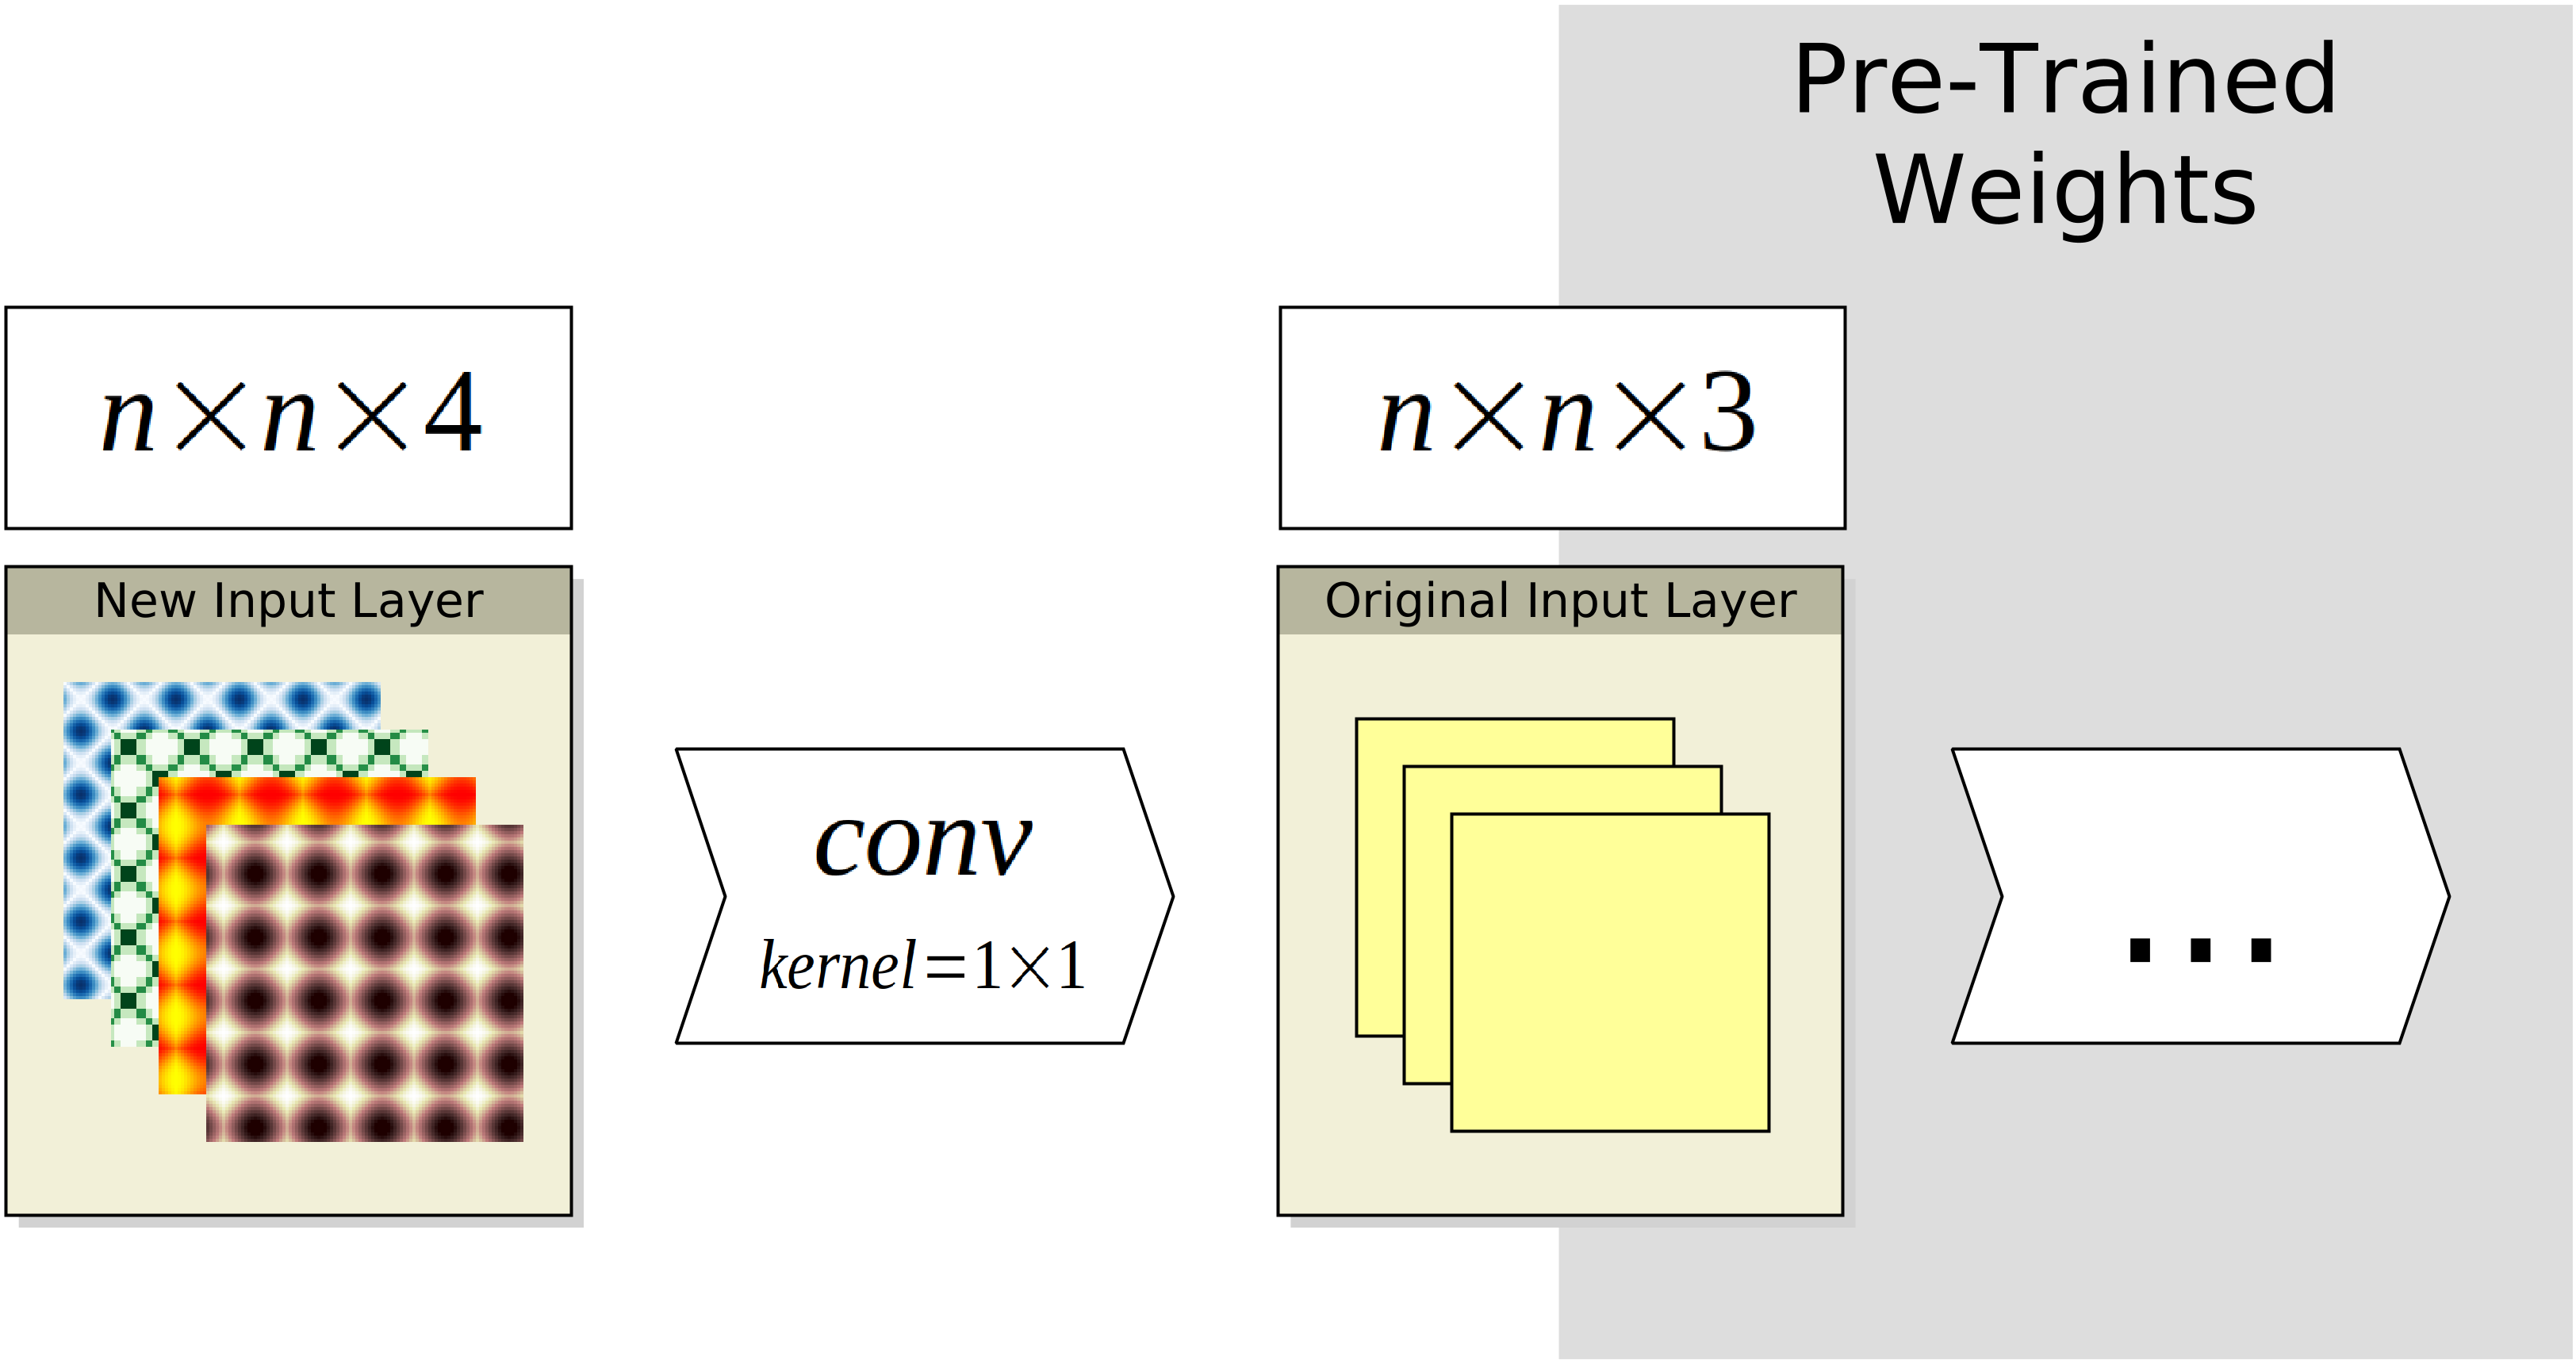
\includegraphics[width=0.8\textwidth]{img/input_layer.png}
	\caption[The three-channeled \acrlong{CV} model feeding process.]{The three-channeled \acrlong{CV} model feeding process. The figure begins in the left, in its input, and progresses to the right. }
	\label{fig:input_layer}
\end{figure}


\begin{figure}[t]
	\centering
	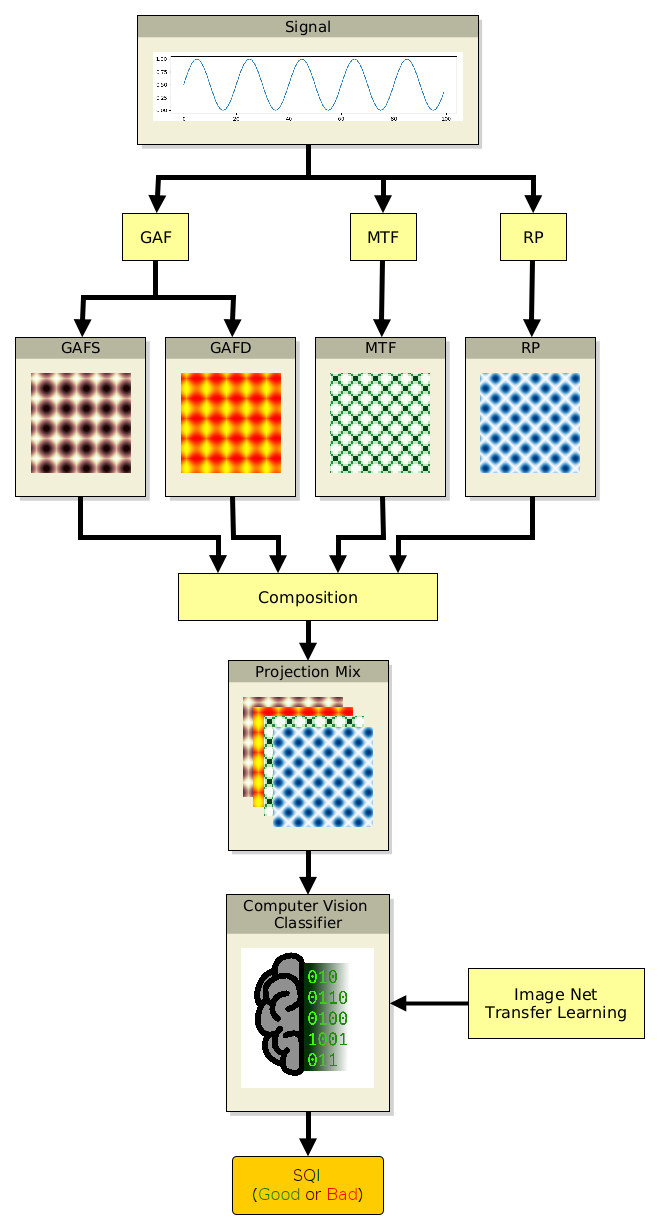
\includegraphics[height=0.95\textheight]{img/method.png}
	\caption{The proposed method. It mainly consisted in feeding the projection composition to the pre-trained \gls{CV} model.}
	\label{fig:method}
\end{figure}


